\section{Theoretical Analysis}
\label{sec:analysis}

\paragraph{} The values used in both analysis are the following:


\begin{table}[h]
  \centering
  \begin{tabular}{|l|r|}
    \hline
    {\bf Name} & {\bf Value} \\ \hline
    $R_1$ & 1.007812 $k\Omega$\\ \hline
$R_2$ & 2.003112 $k\Omega$\\ \hline
$R_3$ & 3.045036 $k\Omega$\\ \hline
$R_4$ & 4.178966 $k\Omega$\\ \hline
$R_5$ & 3.106157 $k\Omega$\\ \hline
$R_6$ & 2.060902 $k\Omega$\\ \hline
$R_7$ & 1.006346 $k\Omega$\\ \hline
$V_S$ & 5.048640 $V$\\ \hline
$C$n& 1.025026 $uF$\\ \hline
$K_b$ & 7.059582 $mS$\\ \hline
$K_d$ & 8.039139 $mS$\\ \hline

  \end{tabular}
  \caption{Circuit data generated by inputing 86639 to the $t2\_datagen.py$ file.}                                                            
  \label{tab:data}                                                      
\end{table}   

\subsection{Analysis for t<0}

\paragraph{} For t<0 we can see that we are working in the steady state, given that in that time interval $v_S$ = $V_S$. In a DC circuit, the capacitor charges up to it's full capacity, blocking the flow of electricity. Taking 
this into account we can replace the capacitor with an open circuit. With this information, and knowing that the the tension in $V_4$, since it is connected to ground, we can obtain the following equations.

\begin{equation}
\begin{bmatrix}
	-1	&	0	&	0	&	0	&	0	&	0	&	0 \\
	G_1	&	-G_1 - G_2 - G_3	&	G_2	&	G_3	&	0	&	0	&	0 \\
	0	&	-K_b - G_2	&	G_2	&	K_b	&	0	&	0	&	0 \\
	G_1	&	-G_1	&	0	&	-G_4	&	0	&	-G_6	&	0 \\
	0	&	0	&	0	&	0	&	0	&	G_6 + G_7	&	-G_7 \\
	0	&	0	&	0	&	-1	&	0	&	-G_6 *	K_d	&	1 \\
	0	&	G_3	&	0	&	-G_3 - G_4 - G_5	&	G_5	&	-G_6	&	0
\end{bmatrix}
\times
\begin{bmatrix}
	V_1 \\
	V_2 \\
	V_3 \\
	V_5 \\
	V_6 \\
	V_7 \\
	V_8
\end{bmatrix}
=
\begin{bmatrix}
	-V_s \\
	0 \\
	0 \\
	0 \\
	0 \\
	0 \\
	0
	\label{m:1}
\end{bmatrix}
\end{equation}

After solving them with the Octave sofware, we obtained the following results:



\begin{table}[h]
  \centering
  \begin{tabular}{|l|r|}
    \hline
    {\bf Name} & {\bf Value} \\ \hline
    $V1$ & 5.064003 $V$\\ \hline
$V2$ & 4.796768 $V$\\ \hline
$V3$ & 4.214280 $V$\\ \hline
$V5$ & 4.836582 $V$\\ \hline
$V6$ & 5.686007 $V$\\ \hline
$V7$ & -1.826284 $V$\\ \hline
V8 & -2.782939 $V$\\ \hline
$I(R_1)$ & 0.266711 $mA$\\ \hline
$I(R_2)$ & 0.279731 $mA$\\ \hline
$I(R_3)$ & 0.013020 $mA$\\ \hline
$I(R_4)$ & 1.178228 $mA$\\ \hline
$I(R_5)$ & 0.279731 $mA$\\ \hline
$I(R_6)$ & 0.911517 $mA$\\ \hline
$I(R_7)$ & 0.911517 $mA$\\ \hline
$I(V_s)$ & 0.266711 $mA$\\ \hline
$I_b$ & -0.279731 $mA$\\ \hline
$I_c$ & 0.000000 $mA$\\ \hline
$I(K_d)$ & 0.911517 $mA$\\ \hline

  \end{tabular}
  \caption{Nodal Analysis for $t<0~s$. Currents are expressed in milliAmpere and Voltages are expressed in Volt.}                                                            
  \label{tab:theoretical1}                                                      
\end{table}   



\subsection{Equivalent Resistance and Initial Conditions}


\paragraph{}In order to determine the equivalent resistance we need to determine $V_X$, this is, the difference between $V_6$ - $V_8$. This is made to ensure that the voltage in the capacitor is continuous.

Making use of the matrix below:

\begin{equation}
\begin{pmatrix}
-1 & 0 & 0 & 0 & 0 & 0 & 0\\
G1 & -G1-G2-G3 & G2 & G3 & 0 & 0 & 0\\
0 & -Kb-G2 & G2 & Kb & 0 & 0 & 0\\
G1 & -G1 & 0 & -G4 & 0 & -G6 & 0\\
0 & 0 & 0 & 0 & 0 & G6+G7 & -G7\\
0 & 0 & 0 & -1 & 0 & -G6*Kd & 1\\
0 & 0 & 0 & 0 & -1 & 0 & 1\\
\end{pmatrix}
\begin{pmatrix}
V1\\
V2\\
V3\\
V5\\
V6\\
V7\\
V8\\
\end{pmatrix}
=
\begin{pmatrix}
0\\
0\\
0\\
0\\
0\\
0\\
-Vx\\
\end{pmatrix}
\end{equation}
\newpage
And knowing that:

\begin{equation}
	V_x = V_6 - V_8
\end{equation}

\begin{equation}
	I_x = \frac{V_6 - V_5}{R_5} + \frac{V_3 - V_2}{R_2}
\end{equation}

\begin{equation}
	R_eq = \frac{V_x}{I_x}
\end{equation}

\begin{equation}
	\tau = R_eq * C
\end{equation}

We can obtain the following values:

\begin{table}[h]
  \centering
  \begin{tabular}{|l|r|}
    \hline    
    {\bf Name} & {\bf Value} \\ \hline
    $V_x$ & 8.468946 $V$\\ \hline
$I_x$ & 2.788975 $mA$\\ \hline
$R_{Eq}$ & 3.036581 $k\Omega$\\ \hline
$\tau$ & 0.003096 $s$\\ \hline 
  \end{tabular}
  \caption{Second nodal analysis and calculations for $R_{Eq}$ and $\tau$. Currents are expressed in $milliAmpere$, Voltages are expressed in $Volt$, Resistances are expressed in $kiloOhm$ and Time Constant is expressed in $second$.}
  \label{tab:theoretical2}
\end{table}

\subsection{Natural Solution}


\paragraph{} The natural solution doesn't take into account independent power sources. Using $V_x$ as the initial condition the natural solution can be obtained with the following equation

\begin{equation}
	V_{6n}(t) = V_x e^{(-\frac{t}{\tau})}
\end{equation}

After computing this data on Octave, we can plot the results of the interval [0, 20]ms.


\begin{figure}[h] \centering
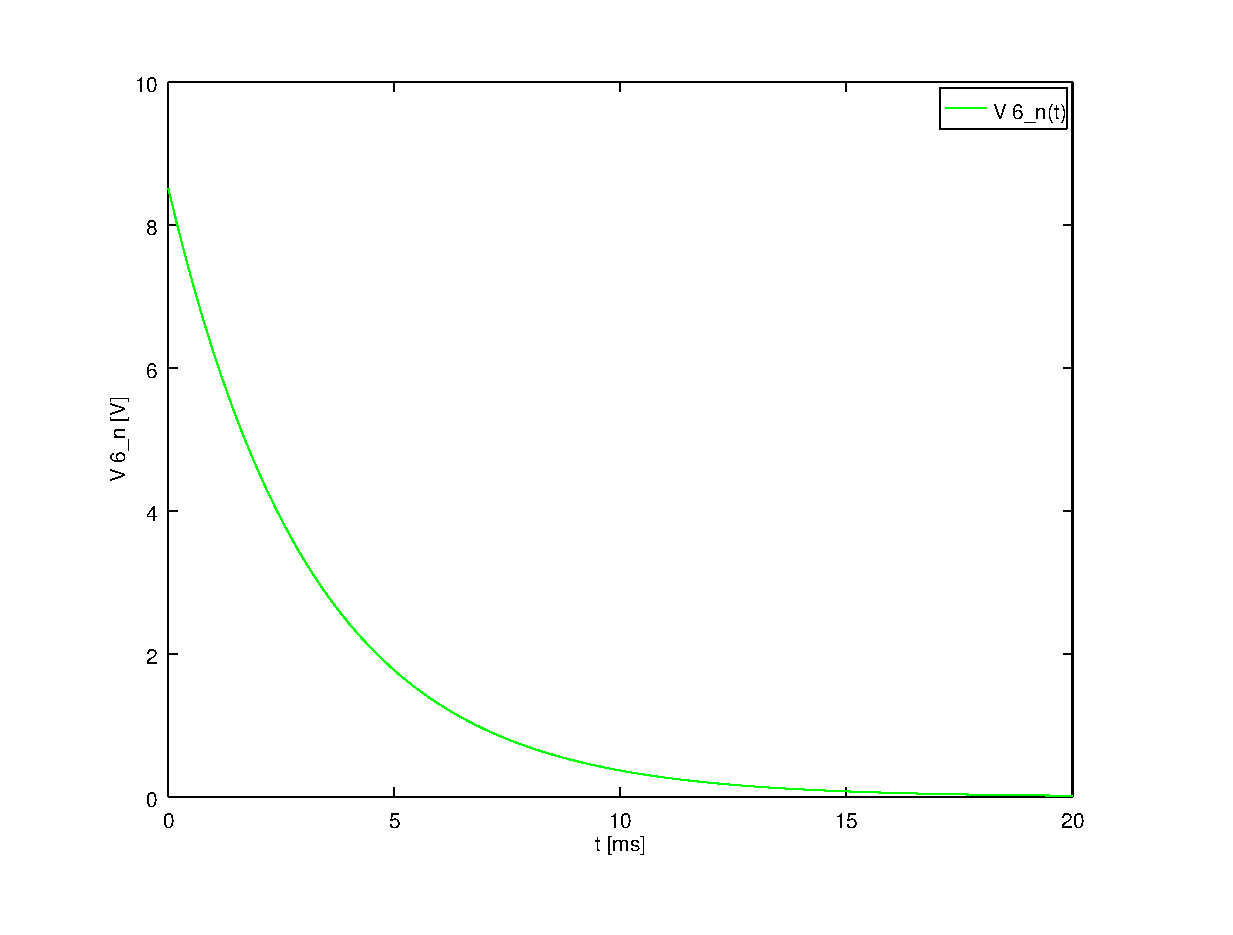
\includegraphics[width=0.6\linewidth]{natural.eps}
	\caption{Natural solution $V_{6n}$ in the interval $[0, 20]~ms$ plot.}
\label{fig:natural}
\end{figure}


\subsection{Forced Solution}

T\paragraph{} In order to obtain the forced solution we must be able to solve the following equation.  

\begin{equation}
\begin{pmatrix}
1 & 0 & 0 & 0 & 0 & 0 & 0\\
-G1 & G1+G2+G3 & -G2 & -G3 & 0 & 0 & 0\\
0 & Kb+G2 & -G2 & -Kb & 0 & 0 & 0\\
-G1 & G1 & 0 & G4 & 0 & G6 & 0\\
0 & 0 & 0 & 0 & 0 & -G6-G7 & G7\\
0 & 0 & 0 & 1 & 0 & G6*Kd & -1\\
0 & -G3 & 0 & G3+G4+G5 & -G5-jwC & G6 & jwC\\
\end{pmatrix}
\begin{pmatrix}
V1\\
V2\\
V3\\
V5\\
V6\\
V7\\
V8\\
\end{pmatrix}
=
\begin{pmatrix}
-j\\
0\\
0\\
0\\
0\\
0\\
0\\
\end{pmatrix}
\end{equation}


The solution to this system is presented in the table below:


\begin{table}[h]
  \centering
  \begin{tabular}{|l|r|r|}
    \hline    
    {\bf Name} & {\bf Complex Amplitude [V]} & {\bf Phase [Degrees]}\\ \hline
    $V_{1}$ & 1.000000 & -90.000000\\ \hline
$V_{2}$ & 0.947229 & -90.000000\\ \hline
$V_{3}$ & 0.832203 & -90.000000\\ \hline
$V_{5}$ & 0.955091 & -90.000000\\ \hline
$V_{6}$ & 0.551847 & 98.938374\\ \hline
$V_{7}$ & 0.360640 & 90.000000\\ \hline
$V_{8}$ & 0.549553 & 90.000000\\ \hline 
  \end{tabular}
  \caption{Nodal analysis for phasor voltage in forced state.}
  \label{tab:phasor}
\end{table}


These values are needed to determine the forced solution $V_{6f}$, which is given by the following formula:

\begin{equation}
V_{6f}(t)=V_{6r}cos(\omega t+V_{6\phi});
\end{equation}

Where

\begin{equation}
\omega=2\pi f;
\end{equation}


\subsection{Final Total Solution}


The final total solution $V_6(t)$ is achieved by superimposing the natural and forced solutions. 



\begin{equation}
	V_6(t)=V_{6n}(t)+V_{6f}(t);
\end{equation}
By converting the phasors to real time functions for $f = 1 kHz$ and superimposing the natural and forced solutions, we can plot both $V_S(t)$ and $V_6(t)$ in the interval $[-5, 20]~ms$, as shown in the figure below:


\begin{figure}[h] \centering
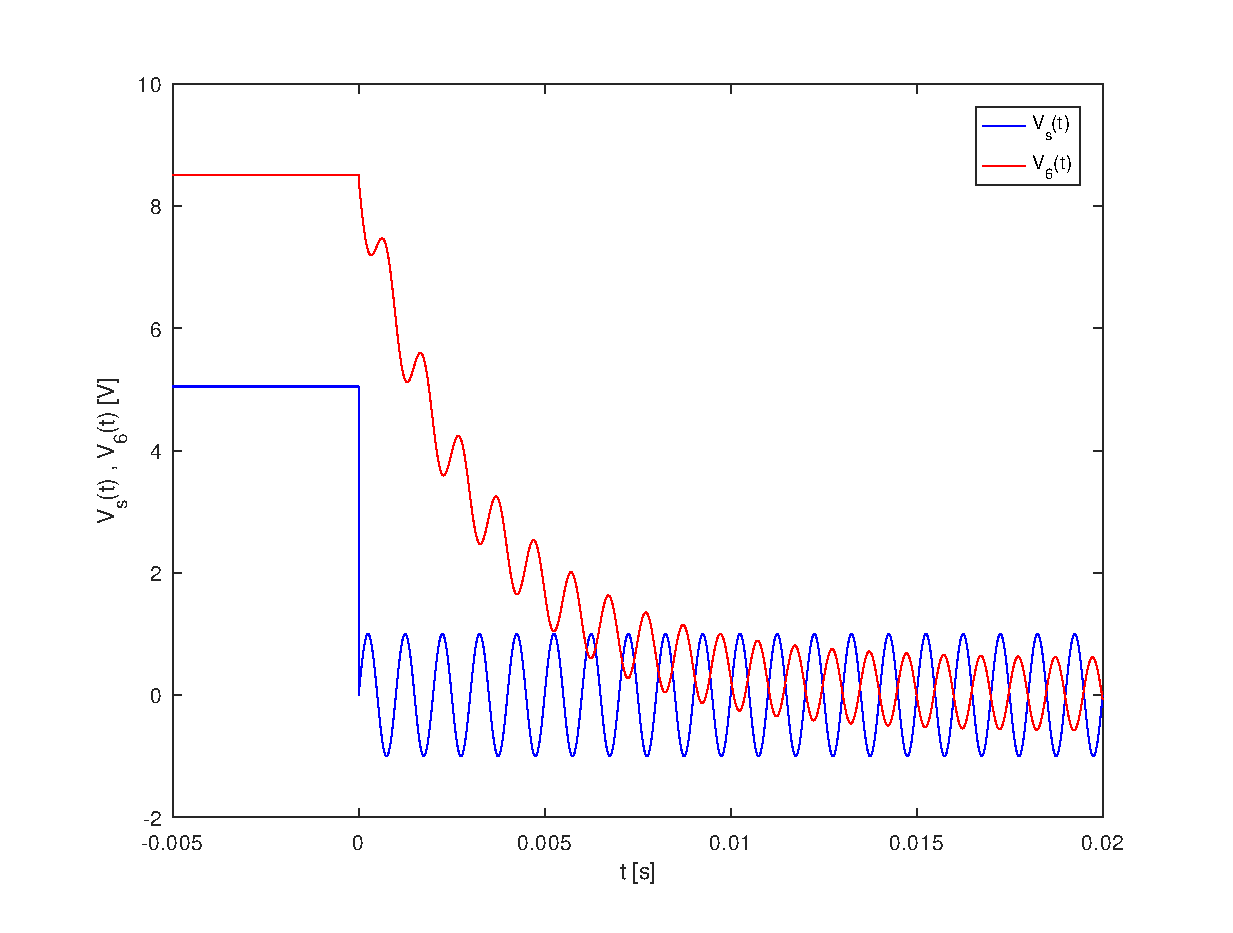
\includegraphics[width=0.7\linewidth]{total.eps}
\caption{Total solution of $V_{6}$ and $V_{s}$ plot.}
	\label{fig:total}
\end{figure}

As expected, both curves shown in Figure~\ref{fig:total} are constant for $t<0~s$. For $t>0~s$, we can see an evident negative exponencial behavior and an induced frequency in $V_{6}$.


\subsection{Frequency Responses}

Because $V_S(t) = sin(\omega t)$, the magnitude and phase are independent of the frequency $f$. This means that both the magnitude and phase are expected to be constant in the plots that follow.

The magnitude frequency response is given in Figure~\ref{fig:mag}.
The phase response for frequencies ranging from $0.1~Hz$ to $1~MHz$ is given in Figure~\ref{fig:phase}. The apparent discontinuity showed in the phase of $V(6)$ is in fact caused by the domain of the arctan function that is used to determined the phase, which is, in reality, continuous.

\begin{figure}[h] \centering
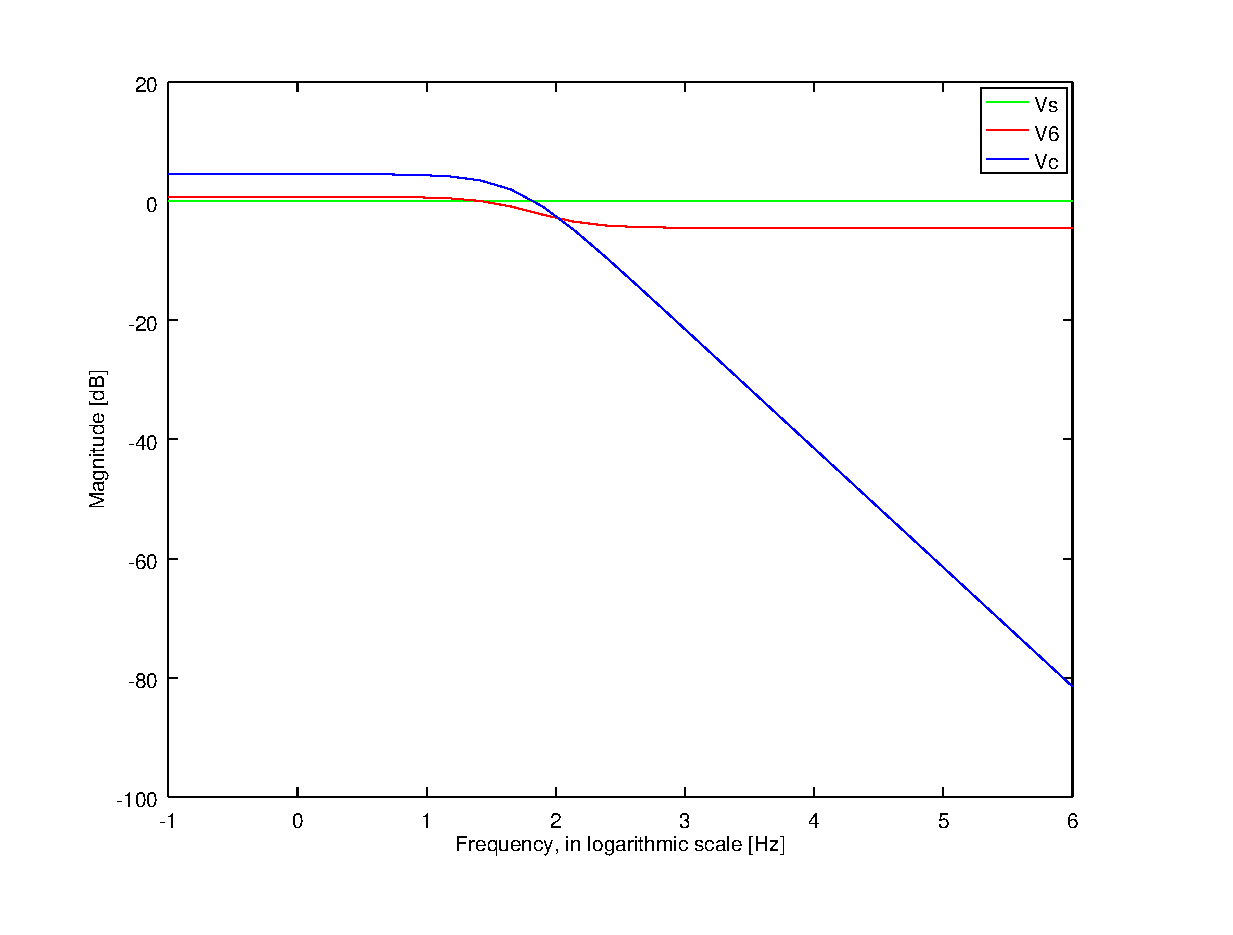
\includegraphics[width=0.5\linewidth]{magnitude.eps}
	\caption{Magnitude frequency response plot, in dB, of $V_{c}$, $V(6)$ and $V_{s}$. Frequencies ranging from $0.1~Hz$ to $1~MHz$ in logarithmic scale.}
        \label{fig:mag}
\end{figure}


\begin{figure}[h] \centering
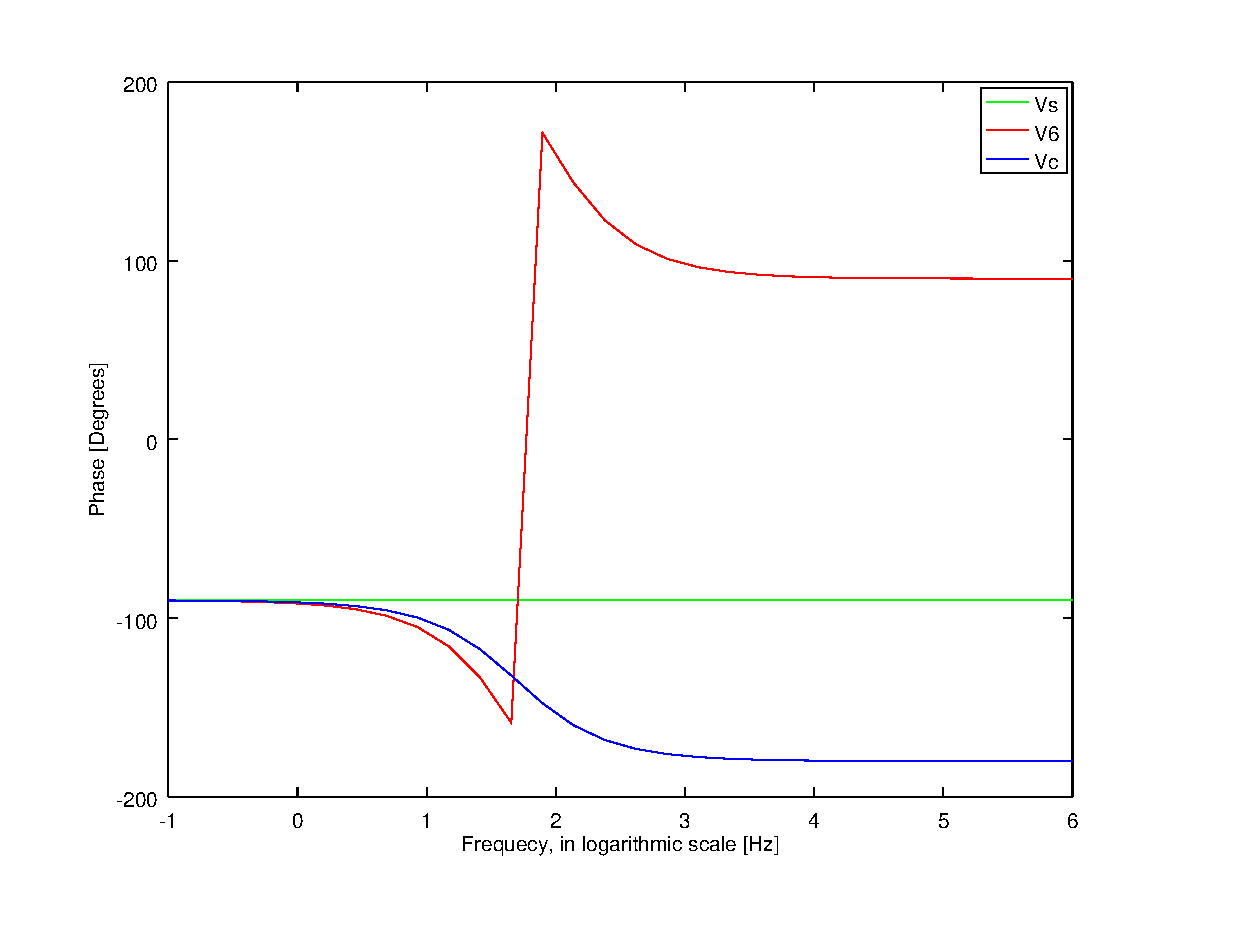
\includegraphics[width=0.7\linewidth]{phase.eps}
	\caption{Phase response plot, in degrees, of $V_{c}$, $V(6)$ and $V_{s}$. Frequencies ranging from $0.1~Hz$ to $1~MHz$ in logarithmic scale.}
        \label{fig:phase}
\end{figure}



The circuit being analysed can be used as a low-pass filter. This means that, for low frequencies, the capacitator has time to charge up to almost the same voltage provided as input (it approximates to an open-circuit behavior), which translates to a proximity in phase between the voltage in the capacitor and the voltage source. Having said that, high frequencies, on the other hand, will give the capacitor a small time to charge up before a change in the input direction occurs (it approximates to a short-circuit behavior), which translates to a growing difference in phase between the voltage in the capacitor and the voltage source. This difference of phase is noticeable for frequencies greater than the cut-off frequency, $f_c$, which is given by $f_c = \frac{1}{2\pi\tau}$. In this particular case, the cut-off frequency value is approximately $50~Hz$. This is why we see a significant voltage drop in Fig~\ref{fig:mag} at around $10~Hz$ and $10^2~Hz$. The phase difference also starts to increase in that same range, as seen in Fig~\ref{fig:phase}.

By simplifying this circuit to an equivalent one composed by a voltage source, capacitor and equivalent resistor, we reach the following equations that help us to better comprehend the magnitude drop and the phase difference rise with the increase of frequency:

\begin{equation}
  V_c = \frac{V_s}{\sqrt{1 + (R_{Eq}\times C\times 2\pi\times f)^2}}
  \label{eq:equivalent1}
\end{equation}

\begin{equation}
  \phi_{V_c} = -\frac{\pi}{2} + arctan(R_{Eq}\times C\times 2\pi\times f)
  \label{eq:equivalent2}
\end{equation}

